\documentclass{article}
\usepackage{graphicx,tikz} 

\title{Directed Acyclic Graphs (DAGs)}
\author{}
\date{December 2024}

\begin{document}

\maketitle % Displays the title, author, and date
\clearpage
% FIRST DAG
\begin{figure}[h!]
\centering
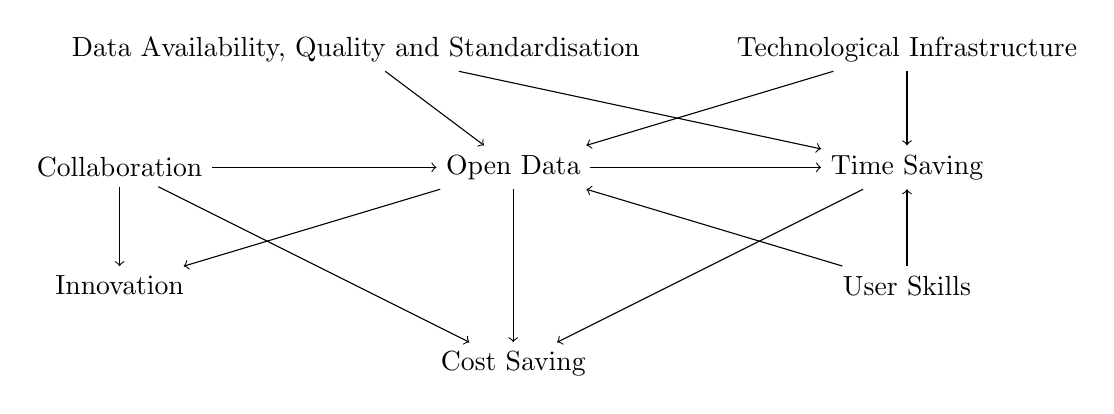
\begin{tikzpicture}

% Nodes
\node (v0) at (-3, -1.5) {Open Data};
\node (v1) at (-3,-4) {Cost Saving};
\node (v2) at (2, -1.5) {Time Saving};
\node (v3) at (2,-3) {User Skills};
\node (v4) at (-8, -3) {Innovation};
\node (v5) at (-8, -1.5) {Collaboration};
\node (v6) at (2, 0) {Technological Infrastructure};
\node (v7) at (-5, 0) {Data Availability, Quality and Standardisation};

% Arrows
\draw[->] (v7) -- (v0);
\draw[->] (v6) -- (v0);
\draw[->] (v5) -- (v0);
\draw[->] (v0) -- (v1);
\draw[->] (v0) -- (v2);
\draw[->] (v5) -- (v4);
\draw[->] (v0) -- (v4);
\draw[->] (v5) -- (v1);
\draw[->] (v2) -- (v1);
\draw[->] (v3) -- (v0);
\draw[->] (v3) -- (v2);
\draw[->] (v6) -- (v2);
\draw[->] (v7) -- (v2);

\end{tikzpicture}
\caption{First DAG}
\label{fig:first_dag}
\end{figure}

\clearpage

% SECOND DAG
\begin{figure}[h!]
\centering
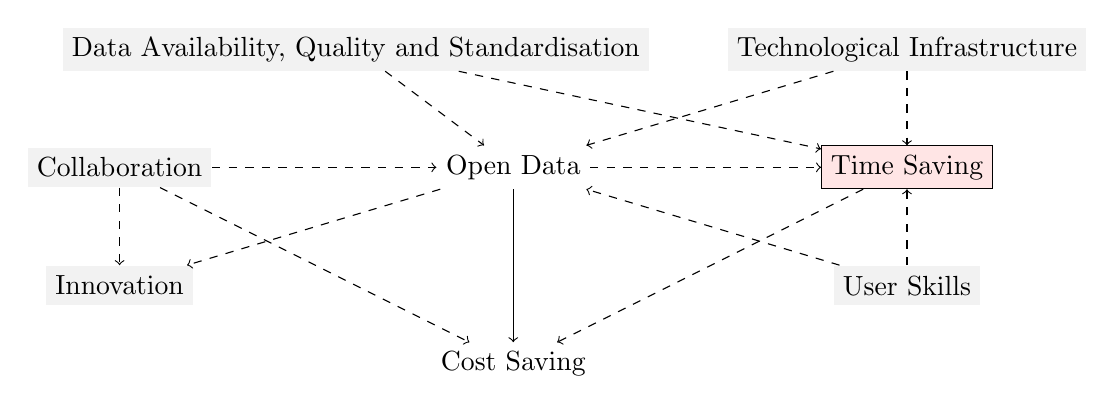
\begin{tikzpicture}[
    box/.style={rectangle, fill=gray!10, minimum height=0.5cm, minimum width=1.5cm},
    highlight/.style={rectangle, draw, fill=red!10, minimum height=0.5cm, minimum width=1.5cm}
]

% Nodes
\node (v0) at (-3, -1.5) {Open Data};
\node (v1) at (-3,-4) {Cost Saving};
\node[highlight] (v2) at (2, -1.5) {Time Saving};
\node[box] (v3) at (2,-3) {User Skills};
\node[box] (v4) at (-8, -3) {Innovation};
\node[box] (v5) at (-8, -1.5) {Collaboration};
\node[box] (v6) at (2, 0) {Technological Infrastructure};
\node[box] (v7) at (-5, 0) {Data Availability, Quality and Standardisation};

% Arrows
\draw[dashed,->] (v7) -- (v0);
\draw[dashed,->] (v6) -- (v0);
\draw[dashed,->] (v5) -- (v0);
\draw[->] (v0) -- (v1);
\draw[dashed,->] (v0) -- (v2);
\draw[dashed,->] (v5) -- (v4);
\draw[dashed,->] (v0) -- (v4);
\draw[dashed,->] (v5) -- (v1);
\draw[dashed,->] (v2) -- (v1);
\draw[dashed,->] (v3) -- (v0);
\draw[dashed,->] (v3) -- (v2);
\draw[dashed,->] (v6) -- (v2);
\draw[dashed,->] (v7) -- (v2);

\end{tikzpicture}
\caption{Second DAG}
\label{fig:second_dag}
\end{figure}

\clearpage

% THIRD DAG
\begin{figure}[h!]
\centering
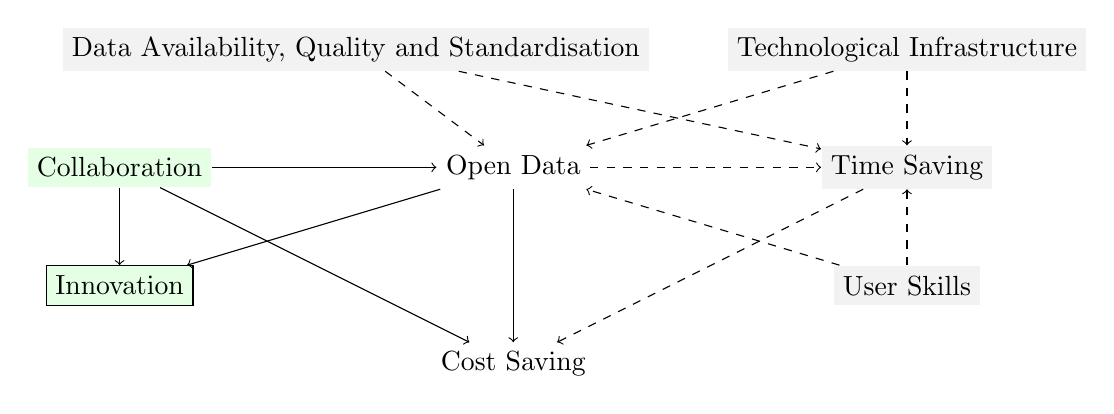
\begin{tikzpicture}[
    node distance=2cm and 3cm,
    every node/.style={align=center},
    box/.style={rectangle, fill=gray!10, minimum height=0.5cm, minimum width=1.5cm},
    highlightGreen/.style={rectangle, draw, fill=green!10, minimum height=0.5cm, minimum width=1.5cm},
    borderHighlight/.style={rectangle, fill=green!10, minimum height=0.5cm, minimum width=1.5cm}
]

% Nodes
\node (v0) at (-3, -1.5) {Open Data};
\node (v1) at (-3,-4) {Cost Saving};
\node[box] (v2) at (2, -1.5) {Time Saving};
\node[box] (v3) at (2,-3) {User Skills};
\node[highlightGreen] (v4) at (-8, -3) {Innovation};
\node[borderHighlight] (v5) at (-8, -1.5) {Collaboration};
\node[box] (v6) at (2, 0) {Technological Infrastructure};
\node[box] (v7) at (-5, 0) {Data Availability, Quality and Standardisation};

% Arrows
\draw[dashed,->] (v7) -- (v0);
\draw[dashed,->] (v6) -- (v0);
\draw[->] (v5) -- (v0);
\draw[->] (v0) -- (v1);
\draw[dashed,->] (v0) -- (v2);
\draw[->] (v5) -- (v4);
\draw[->] (v0) -- (v4);
\draw[->] (v5) -- (v1);
\draw[dashed,->] (v2) -- (v1);
\draw[dashed,->] (v3) -- (v0);
\draw[dashed,->] (v3) -- (v2);
\draw[dashed,->] (v6) -- (v2);
\draw[dashed,->] (v7) -- (v2);

\end{tikzpicture}
\caption{Third DAG}
\label{fig:third_dag}
\end{figure}

\clearpage

% FOURTH DAG
\begin{figure}[h!]
\centering
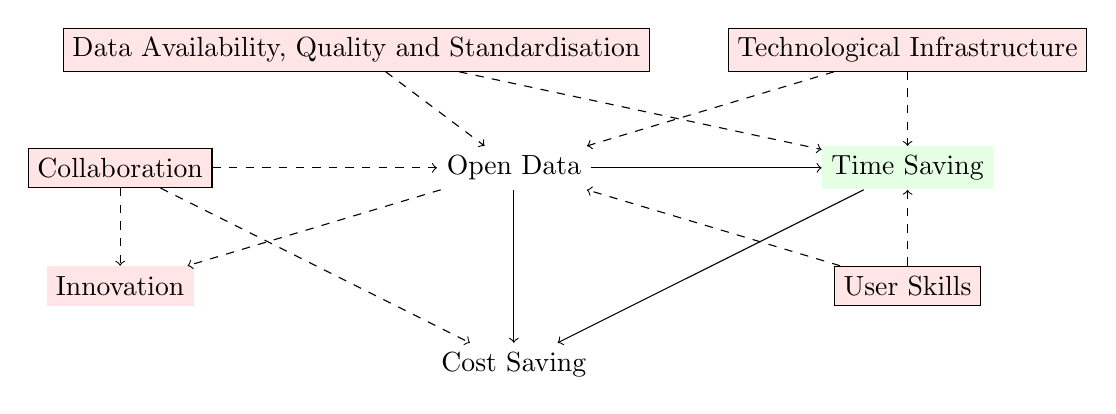
\begin{tikzpicture}[
    node distance=2cm and 3cm,
    every node/.style={align=center},
    box/.style={rectangle, fill=gray!10, minimum height=0.5cm, minimum width=1.5cm},
    borderRed/.style={rectangle, draw, fill=red!10, minimum height=0.5cm, minimum width=1.5cm},
    highlightGreen/.style={rectangle, fill=green!10, minimum height=0.5cm, minimum width=1.5cm},
    highlightRed/.style={rectangle, fill=red!10, minimum height=0.5cm, minimum width=1.5cm}
]

% Nodes
\node (v0) at (-3, -1.5) {Open Data};
\node (v1) at (-3,-4) {Cost Saving};
\node[highlightGreen] (v2) at (2, -1.5) {Time Saving};
\node[borderRed] (v3) at (2,-3) {User Skills};
\node[highlightRed] (v4) at (-8, -3) {Innovation};
\node[borderRed] (v5) at (-8, -1.5) {Collaboration};
\node[borderRed] (v6) at (2, 0) {Technological Infrastructure};
\node[borderRed] (v7) at (-5, 0) {Data Availability, Quality and Standardisation};

% Arrows
\draw[dashed,->] (v7) -- (v0);
\draw[dashed,->] (v6) -- (v0);
\draw[dashed,->] (v5) -- (v0);
\draw[->] (v0) -- (v1);
\draw[->] (v0) -- (v2);
\draw[dashed,->] (v5) -- (v4);
\draw[dashed,->] (v0) -- (v4);
\draw[dashed,->] (v5) -- (v1);
\draw[->] (v2) -- (v1);
\draw[dashed,->] (v3) -- (v0);
\draw[dashed,->] (v3) -- (v2);
\draw[dashed,->] (v6) -- (v2);
\draw[dashed,->] (v7) -- (v2);

\end{tikzpicture}
\caption{Fourth DAG}
\label{fig:fourth_dag}
\end{figure}

\end{document}
